\chapter{Аналитический раздел}
В данном разделе приведено описание решения всех аналитических задач.


\section{Развязывание потоков выполнения сервера}

По заданию в данной работе используются рабочие процессы.
В ~\cite{Krisch1} рассмотрены возможные схемы обслуживание клиентов:

\begin{enumerate}
\item Обслуживание по очереди в одном потоке
\item Многопоточный сервер (по одному потоку на клиента)
\item Вариация c пулом потоков или процессов
\item Использование select() или poll() в одном процессе
\item Опрос неблокирующих сокетов
\end{enumerate}

В соответствии с поставленным заданием была выбрана следующая схема:

При запуске сервера создается определенное в конфигурации число рабочих процессов,
т.е. процессы создаются статически один раз при запуске сервера и уничтожаются при его выключении.
Это позволяет не тратить системные ресурсы на создание и уничножение процессов (в отличие от схемы с динамическим созданием процессов), а также предохраняет от чрезмерного потребления системных ресурсов (в отличие от схем, где на каждого клиента создается отдельный поток или процесс).

Каждый процесс имеет свою очередь обслуживаемых подключений, все сокеты подключений переведены в неблокирующий режим, это позволяет тратить процессу минимум времени на обсуживание одного подключения и не блокироваться при ожидании сообщений, таким образом обслуживая много клиентов единовременно.

В цикле обслуживания каждый процесс использует в соответствии с заданием вызов poll(), что позволяет прослушивать одновременно
все подключения процесса и не тратить ресурсы на их циклический опрос.




\section{Разделение нагрузки между рабочими процессами}
Каждый рабочий процесс в цикле осуществляет вызов poll() и при возврате проверяет listen сокет, если на нем есть новое подключение, процесс пытается принять его вызовом accept(). Таким образом один из рабочих процессов принимает подключение, а остальные получают код ошибки и продолжают обслуживание своей очереди заявок, т.к. все сокеты неблокирующие.
Таким образом рабочий процесс выбирается операционной системой из тех, что осуществляют в момент появления подключения вызов poll().



\section{Сущности предметной области}
Выделение сущностей предметной области представлено на рис.~\ref{fig:er} 


\begin{figure}[ht]
\centering
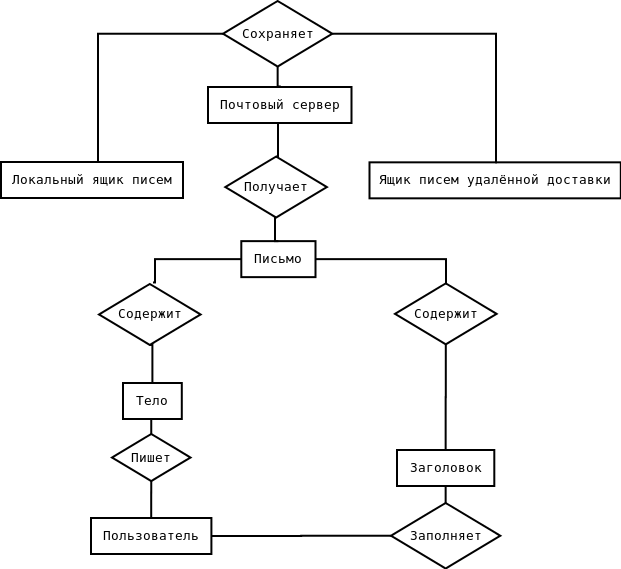
\includegraphics[width=\textwidth]{dia/er.png}
\caption{Сущности предметной области}
\label{fig:er}
\end{figure}





